% FIGURE_INCLUDE_SUGGESTION.tex
% ACM single-column pair layout. Independent captions, no subfigure, no (a)/(b).
% Paths relative to Paper6_ToN/.

% --- Pair 1 ---
\begin{figure}[t]
\noindent
\begin{minipage}[t]{0.495\columnwidth}
  \centering
  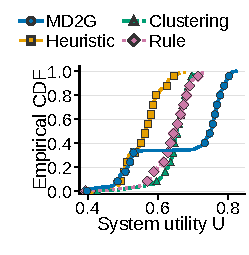
\includegraphics[width=\linewidth]{Figures/QoE/QoE_By_Strategy.pdf}
  \caption{Utility ECDF over development workloads.}
  \label{fig:ton-u-by-strategy}
\end{minipage}\hspace{0.01\columnwidth}%
\begin{minipage}[t]{0.495\columnwidth}
  \centering
  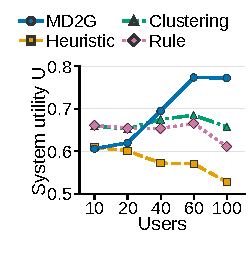
\includegraphics[width=\linewidth]{Figures/Buffer Level/System_Utility_By_Users_scheme1.pdf}
  \caption{Utility versus receiver concurrency.}
  \label{fig:ton-concurrency-crossover}
\end{minipage}
\end{figure}

% --- Pair 2 ---
\begin{figure}[t]
\noindent
\begin{minipage}[t]{0.495\columnwidth}
  \centering
  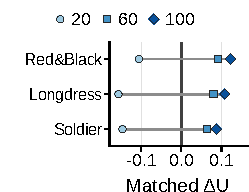
\includegraphics[width=\linewidth]{Figures/QoE/QoE_By_Content_DeltaU.pdf}
  \caption{Content-wise matched $\Delta U$ across loads.}
  \label{fig:ton-delta-by-content}
\end{minipage}\hspace{0.01\columnwidth}%
\begin{minipage}[t]{0.495\columnwidth}
  \centering
  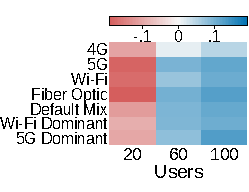
\includegraphics[width=\linewidth]{Figures/QoE/QoE_By_Network.pdf}
  \caption{Network-wise matched $\Delta U$ across loads.}
  \label{fig:ton-delta-by-network}
\end{minipage}
\end{figure}

% --- Pair 3 ---
\begin{figure}[t]
\noindent
\begin{minipage}[t]{0.495\columnwidth}
  \centering
  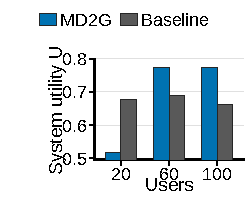
\includegraphics[width=\linewidth]{Figures/QoE/Loot_Holdout_DeltaU_By_Users.pdf}
  \caption{Matched utility on unseen Loot.}
  \label{fig:ton-loot-deltau}
\end{minipage}\hspace{0.01\columnwidth}%
\begin{minipage}[t]{0.495\columnwidth}
  \centering
  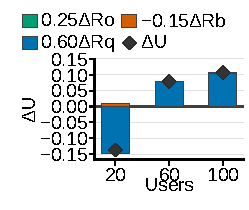
\includegraphics[width=\linewidth]{Figures/QoE/Mechanism_Decomposition_Development.pdf}
  \caption{Matched $\Delta U$ decomposition on the development matrix.}
  \label{fig:ton-mechanism}
\end{minipage}
\end{figure}

% --- Pair 4 ---
\begin{figure}[t]
\noindent
\begin{minipage}[t]{0.495\columnwidth}
  \centering
  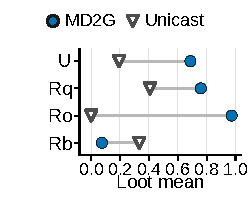
\includegraphics[width=\linewidth]{Figures/QoE/MoQ_Shared_vs_Unicast.pdf}
  \caption{Shared MoQ versus MoQ-Unicast on Loot.}
  \label{fig:ton-shared-vs-unicast}
\end{minipage}\hspace{0.01\columnwidth}%
\begin{minipage}[t]{0.495\columnwidth}
  \centering
  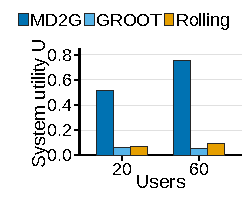
\includegraphics[width=\linewidth]{Figures/User_Experience_Trade-off/H2_Cross_Stack_DASH.pdf}
  \caption{Cross-stack utility at 20 and 60 users.}
  \label{fig:ton-h2-secondary}
\end{minipage}
\end{figure}

% --- Fair live MCG mechanism (figure*; native 7.00×2.20 in; 0.97\textwidth) ---
\begin{figure*}[t]
  \centering
  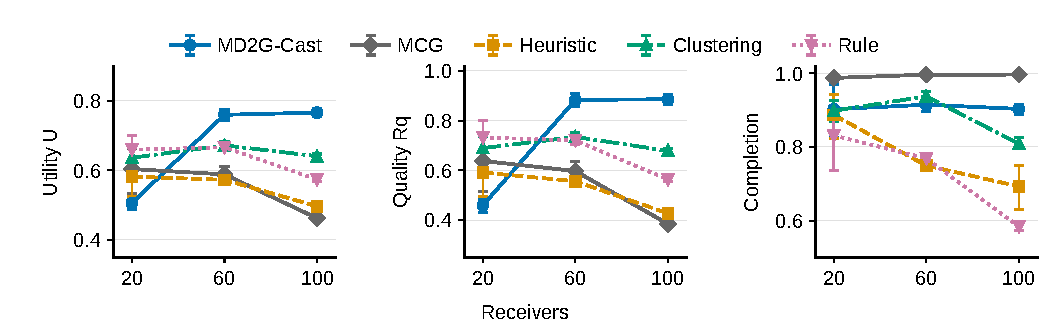
\includegraphics[width=0.97\textwidth]{Figures/QoE/Live_MCG_Fair_Mechanism_1x3.pdf}
  \caption{Focused live same-substrate comparison on Red-and-Black
under 4G, Wi-Fi, and fiber access using three matched seeds.
From left to right, the panels report system utility, decoded
quality \(R_q\), and raw component-completion fraction.
MCG maintains high raw component completion as concurrency grows,
but this does not translate into high decoded service quality.}
  \label{fig:ton-live-mcg-fair}
\end{figure*}

% --- Supporting throughput (protocol-inclusive TX; not efficiency) ---
\begin{figure*}[t]
  \centering
  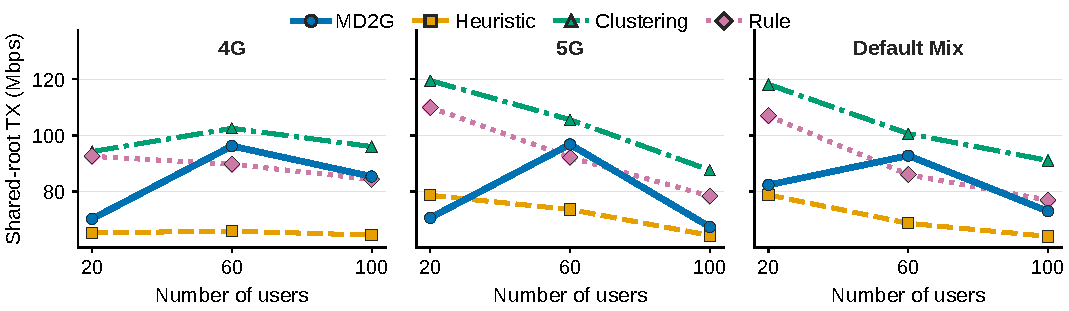
\includegraphics[width=\textwidth]{Figures/Throughput/System_Throughput_MainText_1x3.pdf}
  \caption{Shared-root TX under 4G, 5G, and Default Mix. Supporting load evidence only: lower TX is not higher efficiency.}
  \label{fig:ton-throughput-main}
\end{figure*}
